\subsection{The integral closure of a ring of fractions}

Let A be a ring, R an A-algebra and S a multiplicative subset of A. Recall (Chapter II, § 2, no. 8) that \(\mathbf{S}^{-1}\mathbf{R}\) has a canonical \(\mathbf{S}^{-1}\mathbf{A}\) -algebra structure.

PROPOSITION 16. Let A be a ring, R an A-algebra, A' the integral closure of A in R and S a multiplicative subset of A. Then the integral closure of \(\mathbf{S}^{-1}\mathbf{A}\) in \(\mathbf{S}^{-1}\mathbf{R}\) is \(\mathbf{S}^{-1}\mathbf{A}'\) .

Let \(b / s\) be an element of \(S^{-1}A'\) ( \(s \in S, b \in A'\) ). Since the diagram

\pandocbounded{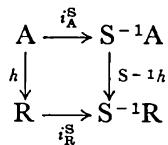
\includegraphics[keepaspectratio]{images/part002_55e4c379.jpg}}

is commutative, \(b / 1\) is integral over \(S^{-1}A\) (no. 1, Proposition 2). As \(1 / s \in S^{-1}A\) , \(b / s = (b / 1)(1 / s)\) is integral over \(S^{-1}A\) .

Conversely, let \(r / t\) ( \(r \in \mathbb{R}\) , \(t \in \mathbb{S}\) ) be an element of \(\mathbf{S}^{-1}\mathbf{R}\) which is integral over \(\mathbf{S}^{-1}\mathbf{A}\) ; then \(r / 1 = (t / 1)(r / t)\) is integral over \(\mathbf{S}^{-1}\mathbf{A}\) . Then there is a relation of the form

\[
(r / 1) ^ {n} + (a _ {1} / s) (r / 1) ^ {n - 1} + \dots + (a _ {n} / s) = 0,
\]

where \(a_{i} \in \mathbf{A}\) ( \(1 \leqslant i \leqslant n\) ) and \(s \in \mathbf{S}\) . This relation may also be written

\[
(s r ^ {n} + a _ {1} r ^ {n - 1} + \dots + a _ {n}) / s = 0
\]

and therefore there exists \(s' \in S\) such that \(s'^{n}(sr^{n} + a_{1}r^{n-1} + \cdots + a_{n}) = 0\) ; we deduce that \((s'sr)^{n} + s'a_{1}(s'sr)^{n-1} + \cdots + s'^{n}s^{n-1}a_{n} = 0\) . By definition therefore \(s'sr \in A'\) , whence \(r/1 \in S^{-1}A'\) and \(r/t \in S^{-1}A'\) .

COROLLARY 1. Let A be an integral domain, A' its integral closure and S a multiplicative subset of A such that \(0 \notin S\) . Then the integral closure of \(S^{-1}A\) is \(S^{-1}A'\) .

The field of fractions R of A is also the field of fractions of \(S^{-1}A\) since \(0 \notin S\) (Chapter II, § 1, no. 1, Remark 7); Proposition 16 is then applied to R.

COROLLARY 2. Let A be an integral domain, K its field of fractions, R an algebra over K and B the integral closure of A in R. The elements of R which are algebraic over K (no. 1, Example 1) are the elements of the form \(a^{-1}b\) where \(b \in \mathbf{B}\) and \(a \in \mathbf{A}\) , \(a \neq 0\) ; if L is the algebraic closure of K in R, there exists a basis of L over K contained in B.

The first assertion follows from Proposition 16 applied in the case \(\mathbf{S} = \mathbf{A} - \{0\}\) . If \((x_{i})_{i\in I}\) is a basis of \(\mathbf{L}\) over \(\mathbf{K}\) , then there exists for all \(i\in I\) an element \(a_{i}\neq 0\) of \(\mathbf{A}\) such that \(a_{i}x_{i}\in \mathbf{B}\) ; then \((a_{i}x_{i})_{i\in I}\) is also a basis of \(\mathbf{L}\) over \(\mathbf{K}\) .

COROLLARY 3. Let A be an integral domain and \(\Omega\) the set of maximal ideals of A. For A to be integrally closed, it is necessary and sufficient that, for all \(\mathfrak{m} \in \Omega\) , \(\mathbf{A}_{\mathfrak{m}}\) be integrally closed.

It follows from Corollary 1 that the condition is necessary. The condition is sufficient, for \(\mathbf{A} = \bigcap_{m \in \Omega} \mathbf{A}_m\) (Chapter II, §3, no. 3, formula (2)) and it is sufficient to apply the Corollary to Proposition 8 of no. 2.

COROLLARY 4. Let A be an integral domain, K its field of fractions and S a multiplicative subset of A such that \(0 \notin S\) .

\begin{enumerate}
\def\labelenumi{(\roman{enumi})}
\item
  Let B be a subring of K which is integral over A and let f be the annihilator of the A-module B/A. Then \(S^{-1}f\) is contained in the annihilator of the \((S^{-1}A)\) -module \(S^{-1}B/S^{-1}A\) and is equal to this annihilator if B is a finitely generated A-module.
\item
  Let A' be the integral closure of A. For \(S^{-1}A\) to be integrally closed, it is sufficient that the annihilator f of the A-module A'/A meet S. This condition is also necessary if A' is a finitely generated A-module.
\setcounter{enumi}{0}
\item
  As \(\mathfrak{f}\mathbf{B} \subset \mathbf{A}\) , \((\mathrm{S}^{-1}\mathfrak{f})(\mathrm{S}^{-1}\mathbf{B}) \subset \mathrm{S}^{-1}\mathbf{A}\) and hence \(\mathrm{S}^{-1}\mathfrak{f}\) is contained in Ann \((\mathrm{S}^{-1}\mathrm{B} / \mathrm{S}^{-1}\mathrm{A})\) . If \(\mathbf{B}\) is a finitely generated A-module, the equation \(\mathrm{S}^{-1}\mathfrak{f} = \operatorname{Ann}(\mathrm{S}^{-1}\mathrm{B} / \mathrm{S}^{-1}\mathrm{A})\) is a special case of formula (9) of Chapter II, § 2, no. 4, \(\mathrm{S}^{-1}\mathrm{B} / \mathrm{S}^{-1}\mathrm{A}\) being canonically identified with \(\mathrm{S}^{-1}(\mathrm{B} / \mathrm{A})\) .
\item
  By Corollary 1 \(\mathbf{S}^{-1}\mathbf{A}'\) is the integral closure of \(\mathbf{S}^{-1}\mathbf{A}\) . As the relations \(\mathfrak{f} \cap \mathbf{S} \neq \varnothing\) and \(\mathbf{S}^{-1}\mathfrak{f} = \mathbf{S}^{-1}\mathbf{A}\) are equivalent (Chapter II, § 2, no. 5, Remark) (ii) is an immediate consequence of (i).
\end{enumerate}

If B is a subring of K which is integral over A, the annihilator f of B/A (equal by definition to the transporter A: B (Chapter I, § 2, no. 10)) is sometimes called the conductor of B in A.

COROLLARY 5. Let A be an integral domain, A' its integral closure and f the annihilator of the A-module A'/A. Suppose that A' is a finitely generated A-module. The prime ideals p of A such that A \(_{p}\) is not integrally closed are those which contain f.

This follows immediately from Corollary 4 (ii) applied to S = A - p.

Note that under the hypotheses of Corollary 5 f ≠ 0 since A' is a finitely generated A-module and every element of K/A (K the field of fractions of A) has an annihilator ≠ 0.

* In algebraic geometry, Corollary 5 and the above remark show that the points where an affine variety V is not normal form a closed set distinct from V. *

